% 2019 江苏卷 第17题 题图：单圆锥曲线与少量直线
% 椭圆 x^2/4 + y^2/3 = 1，圆 F2: (x-1)^2 + y^2 = 16
% A(1,4), D(1,3/2), B(-11/5,-12/5), E(-1,-3/2)
\usetikzlibrary{arrows.meta}
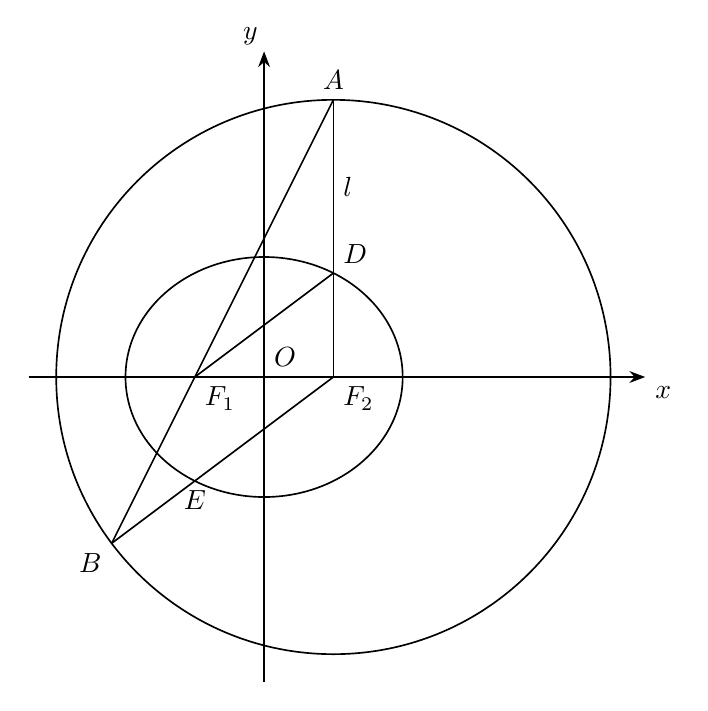
\begin{tikzpicture}[x=0.88cm,y=0.88cm,line width=.6pt,font=\normalsize,>=Stealth]
\def\ellA{2.00000000}
\def\ellB{1.73205081}
\def\circR{4.00000000}
\coordinate (O) at (0.00000000,0.00000000);
\coordinate (F1) at (-1.00000000,0.00000000);
\coordinate (F2) at (1.00000000,0.00000000);
\coordinate (A) at (1.00000000,4.00000000);
\coordinate (D) at (1.00000000,1.50000000);
\coordinate (B) at (-2.20000000,-2.40000000);
\coordinate (E) at (-1.00000000,-1.50000000);
\draw[->] (-3.40000000,0.00000000)--(5.50000000,0.00000000) node[below right] {$x$};
\draw[->] (0.00000000,-4.40000000)--(0.00000000,4.70000000) node[anchor=south east,inner sep=0pt,xshift=-2pt,yshift=2pt] {$y$};
\draw (O) ellipse ({\ellA} and {\ellB});
\draw (F2) circle ({\circR});
\draw (A)--(B);
\draw (B)--(F2);
\draw (D)--(F1);
\draw (A)--(F2);
\node[above right] at (O) {$O$};
\node[below right] at (F1) {$F_1$};
\node[below right] at (F2) {$F_2$};
\node[above] at (A) {$A$};
\node[above right] at (D) {$D$};
\node[below left] at (B) {$B$};
\node[below] at (E) {$E$};
\node[right] at (1.00000000,2.75000000) {$l$};
\end{tikzpicture}
